\documentclass{article}
\usepackage[utf8]{inputenc}
\usepackage{graphicx}
\usepackage{tikz}
\usepackage{todonotes}
\usepackage{hyperref}
\usetikzlibrary{arrows, arrows.meta}
\usepackage{float}
\usepackage[]{algorithm2e}
\usepackage{pgfplots}
\usepackage[cache=false,outputdir=.texpadtmp]{minted}

% Use standard A4 paper and standard margins for A4.
\usepackage[a4paper, margin=2.54cm]{geometry}

\begin{document}
\begin{titlepage}
    \begin{center}
       \vspace*{4cm}

       \textbf{\LARGE Tetris Project for AOS}

       \vspace{1.5cm}
        Design Document for the Tetris project for the course "Advanced Operating System".
            
       \vfill

       \textbf{Authors:}\\
       Accordi Gianmarco\\
       Chierici Franco

       \vspace{0.8cm}
     
       
\includegraphics[width=0.4\textwidth]{img/Logo_Politecnico_Milano.png}
            
       Dipartimento di Elettronica, Informazione e Bioingegneria\\
       Politecnico di Milano\\
       Italy\\
       29/03/2021
            
   \end{center}
\end{titlepage}

\tableofcontents

\newpage

\section{Introduction}
The scope of this document is to explain the design choice we have have made during the development of our project: a version of Tetris working from a terminal console, that is executed on an external microcontroller integrated circuit. 
It will also contains all the reference to better understand the structure of the code.

\section{Design}

\subsection{Interfaces Diagram}
\begin{figure}[H]
    \centering
    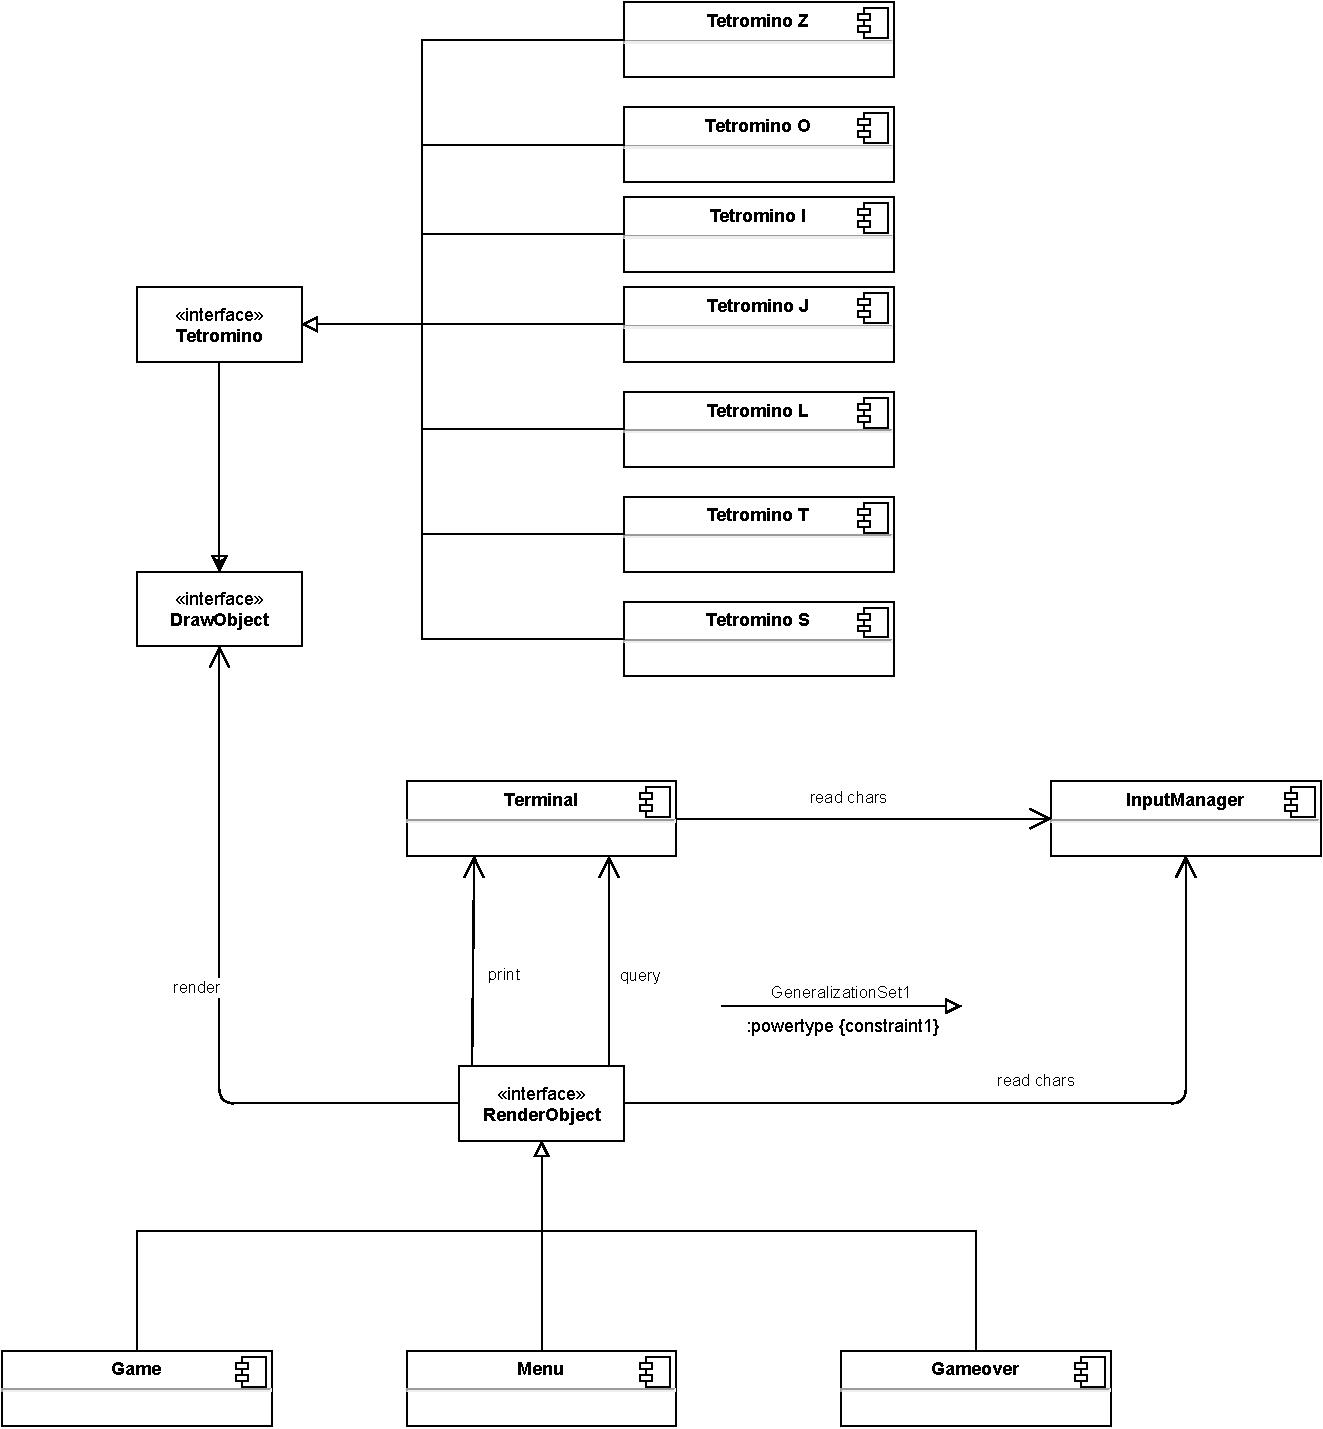
\includegraphics[width=\linewidth]{img/InterafcesDiagram.pdf}
    \caption{Interfaces Diagram of the project.}
    \label{fig:interface}
\end{figure}
The previous diagram \ref{fig:interface} shows the high level structure of project. From it you can see that there are two relevant classes: the \textit{Terminal} and the \textit{InputManager}.
They are two implementation dependent classes that has been introduced in order to decouple the main project logics from the actual platform used.
The \textbf{Terminal} is used to query the terminal used in order to get the available space on the terminal screen, sets the terminal mode, and to print object on it, as further detailed inside \ref{terminal-rendering}.
When needed the following functions are exposed by the Terminal:
\begin{minted}[linenos, bgcolor=white, escapeinside=!!]{c++}
    /* When needed use this method to update the value of col and row */
    int refreshColAndRow();
    /* Set the position of the cursor to the left higher corner of the drawing area, relative
    to the given row and col. */
    void positionCursorForStartDrawing(int posRow, int posCol);
    /* Draw a portion of the screen based on DrawObject
    starting from the position on screen (writingRow, writingCol). */
    void drawOnScreen(DrawObject drawObject, int writingRow, int writingCol);
\end{minted}
The Terminal is instantiate in the entry point of the project that is obviously located at \path{main.cpp}, along with the declaration of the InputManager, than their reference is carried along and passed in the constructor of each
elements that are interested.
The \textbf{InputManager} instead manages the interactions with the user, it collects the characters received from the user in a queue, that is later on read by interested elements (like a \textit{RenderObject}).
\begin{minted}[linenos, bgcolor=white, escapeinside=!!]{c++}
    /* Returns an instance of the last char received from the user.
    NOTE: it is a blocking call. */
    char getLastChar();
    /* Returns an instance of the last char received for the terminal.
    NOTE: it is a blocking call. */
    char getLastCharForTerminal();
\end{minted}
It keeps track of two different queue: one that can be accessed by each element, and the second one only by the terminal. Since we are using ASCII Escape Sequence, we will query the terminal and receive response on the STDIN, so when doing this operation we suspend the adding into the queue of the next char on the STDIN,
and instead we put these chars on the queue for the Terminal, in this way we avoid that the two different streams of chars are mixed altogether.
One of the other Main interfaces is the \textbf{RenderObject}. There will be only one RenderObject at a time, and will be managed by the main code.
As detailed in the \ref{main-loop} each frame we draw is done by calling on the active RenderObject the method:
\begin{minted}[linenos, bgcolor=white, escapeinside=!!]{c++}
    /* Render method of the screen through the Terminal. */
    virtual RenderObject * drawFrame();
\end{minted}
Which draw at each frame what has to be displayed on the screen by the Terminal, that sometimes requires the whole content of the screen to be cleared (call \textit{resetScreen()} on Terminal), or only a portion of it (by using \textit{revertDrawObject()} to undone a previous print, this is done in order to optimize).
The various RenderObject are: \textit{Game}, \textit{Menu}, and \textit{Gameover}.
They all contains the logic used to implement the game.
The other abstraction we have used is to defined the \textbf{DrawObject}, that is an object composed by the following fields:
\begin{minted}[linenos, bgcolor=white, escapeinside=!!]{c++}
    /* Is the string associate to this DrawObject */
    string object_string;
    /* Is the color associate to this DrawObject */
    string color;
\end{minted}
Tha are used by the Terminal when a call to print a DrawObject is done.
The last level of abstraction is represented by the \textbf{Tetromino}, that provides an high level interface, that is extended for each other Tetrominoes. In this way each new Tetrominoes needed requires only to provide a valid constructor that draw the shape of the Tetromino as it was draw on a Grid.
In fact also the state of the Game inside the \textbf{Game} class is saved inside a grid, that when needed is translated inside a DrawObject and sent to the Terminal to be printed.
The definition of the Tetromino class then includes also:
\begin{minted}[linenos, bgcolor=white, escapeinside=!!]{c++}
    /* Returns a string that should be printed on screen. */
    DrawObject toDrawObject();
\end{minted}
that is used in order to get the DrawObject starting from the Tetromino that should be sent to the Terminal to be printed.

\subsection{Sequence Diagram}
\begin{figure}[H]
    \centering
    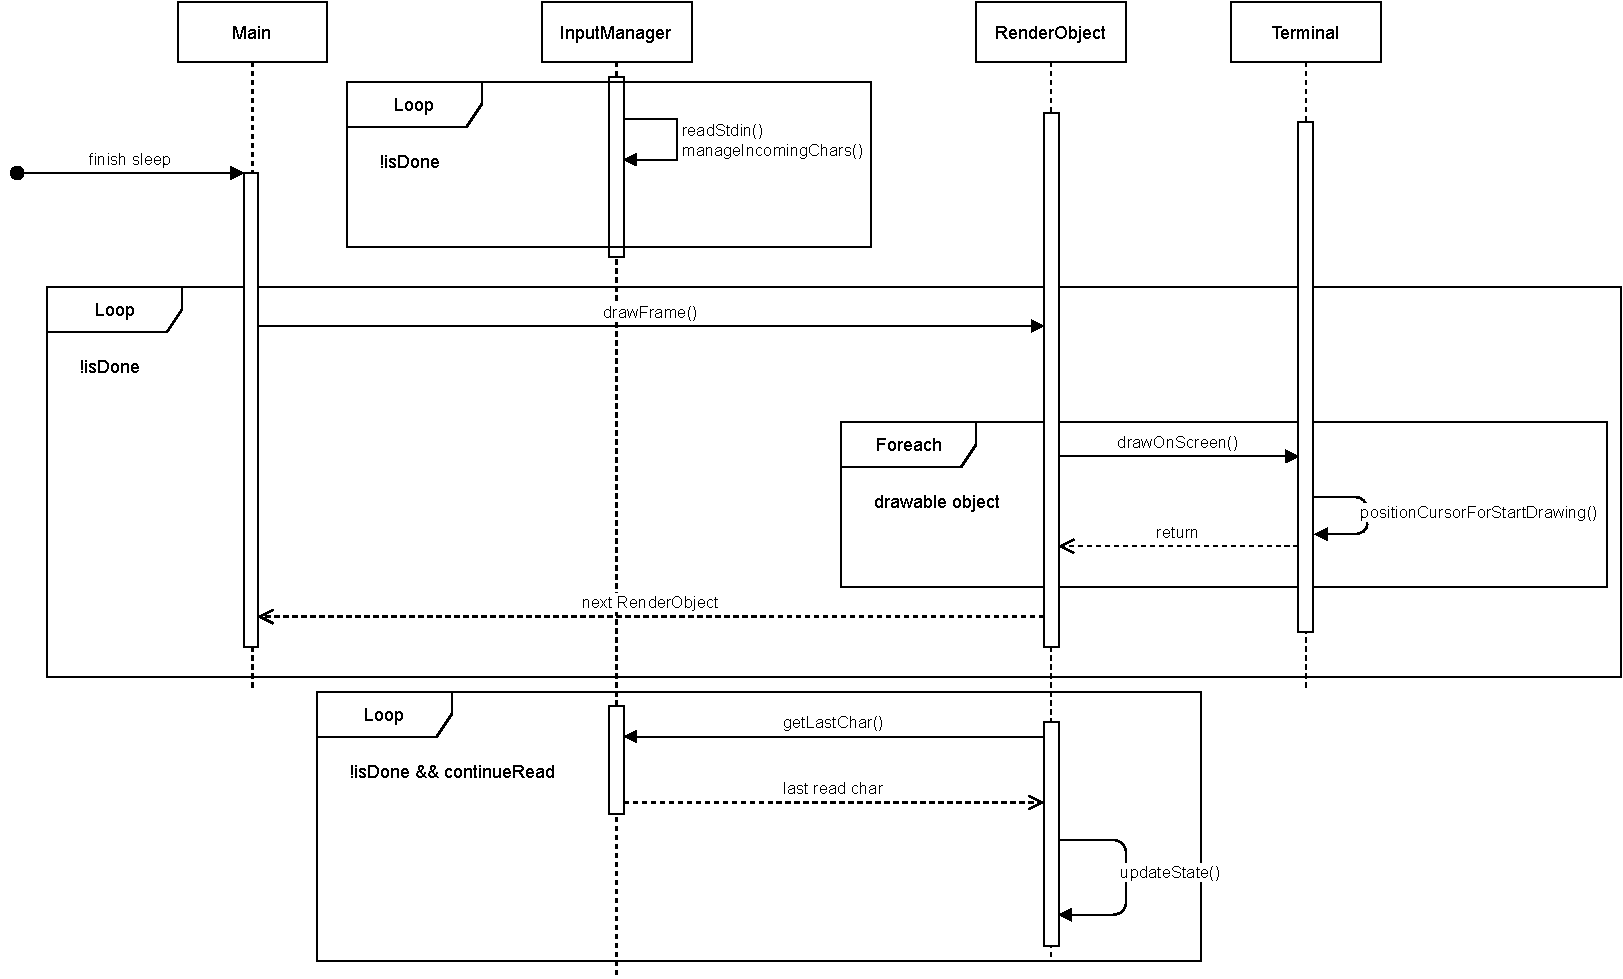
\includegraphics[width=\linewidth]{img/SequenceDiagram.pdf}
    \caption{Sequence Diagram of the project.}
    \label{fig:sequence}
\end{figure}
The above figure better detailed how the components interact among them, and also the interaction with the user.
First of all since we will have different threads that has to coordinate among them, we have defined a global variable inside \path{terminal/utility.h}:
\begin{minted}[linenos, bgcolor=white, escapeinside=!!]{c++}
    extern atomic<bool> isDone;
\end{minted}
In this way when some threads decide to terminate the computation, when for example the user press the quit key, everyone is shutdown correctly, and also the access to the variable is made sequential thanks to the usage of the atomic type.
As said we have adopted a multi-threaded architecture:
\begin{itemize}
    \item the \textbf{InputManager} class has a thread that reads the chars on the stdin and it puts them in the correct queue;
    \item the \textbf{RenderObject} instead has a thread that is used in order to read the chars inside the interested queue from the InputManager, and then it class the \textit{updateState()} method to update the state of the object based on the received char, and it is modeled like a finite state machine;
    \item \textbf{Game} has a thread that has to make update the state of the Tetrominoes used in the game, for example by making a Tetromino sliding down as long as time passes.
\end{itemize}
The figure also highlight three of the main interactions that happens between these components.
For example the first loop is the one of the thread on the InputManager that reads the char from the STDIN;
The second loop is series of invocation that starting from the \label{main-loop}, makes the call to draw the frame based on the actual active RenderObject, that will draw the DrawObject associated to the actual state thanks to the Terminal.
At the end the active RenderObject will returns a next RenderObject different from NULL, if the we have to change the scene, for example when from the Menu the use starts a Game.
The third loop is instead the interaction between the InputManager and the other components interested in getting the last chars from the queues. Because we have defined two queues, one for the chars that are of interest to the RenderObjects and one for the Terminal.
\begin{minted}[linenos, bgcolor=white, escapeinside=!!]{c++}
    const unsigned int defaultSerialSpeed=115200;
\end{minted}
by changing the value of the Baud Rate from 19200 to 115200, this makes the drawing of a scene much faster, since the characters between the board and the PC for example are interchanged more faster.

\section{Target Platform}
Since we have used as target the miosix-kernel, the supported boards are the supported by the kernel itself. We have done most of our work on the STM32 Nucleo-64\footnote{https://www.st.com/en/evaluation-tools/nucleo-l476rg.html}.

\section{Implementation}
This part of the document better highlight what hwo we have proceed in the implementation of our project from a more technical perspective.
To make the refresh procedure works an acceptable velocity we have modified the file under \path{miosix-kernel/miosix/config/arch/cortexM4_stm32l4/stm32l476rg_nucleo/board_settings.h}, and set the 

\subsection{Packages}
Our project has been developed by using C++\cite{slidec++}, in order to be compliant with the miosix-kernel\cite{miosix}.
We choosed C++ over C because we found very useful the object-oriented paradigm. \todo[]{Facciamo confronto tra bare mental e miosix?}

\subsubsection{Miosix}
This OS kernel allowed us to abstract from bare-metal programming and made management of multithreading simple.
\subsubsection{GDB}
The debugger helped us to find bugs and load the program into the board. Also, with the file \emph{.gdbinit} we pre-loaded some base instructions.
\subsubsection{Screen}
Screen is a terminal multiplexer, that allows the board to use a remote terminal session, in this case Ubuntu's terminal.

\subsection{Terminal Rendering}
\label{terminal-rendering}
To render the frames, the first thing we did was to change the terminal mode. Usually it is set in canonical mode, where the program receives the input only when he presses enter.
To achieve a "raw mode", thanks to the library termios, we turned on the local flag ICANON, that sets the terminal to canonical mode, and the ECHO flag.
The ECHO flag tells the terminal to print every key that the user is writing, and by default is on, because normally a user wants to see what is typing.
In order to get the terminal size and reset the screen, we used the ansii escape sequence. TODO

\subsection{Main Loop}
\label{main-loop}
\begin{algorithm}[H]
    Setup of the InputManager and the Terminal\;
    \While{!isDone} {\
        Call drawFrame() on the actualRenderObject\;
        \eIf{the returnedRenderObject!=NULL}{
            update actualRenderObject with the returnedRenderObject\;      
        }
        Sleep for 500 milliseconds\;
    }
    \caption{Main loop executed inside the main.cpp.}
\end{algorithm}
This is the loop executed in the main, that draws a frame every 500ms, thanks to the last sleep.
It maintains update the actualRenderObject based on the value returned by the RenderObject upon updating the scene.
After rendering the scene in the last frame, the main awaits for 500 milliseconds, and then it stops its computation if someone has update the value of isDone to true, if for example the user has pressed the quit key.
Another important part is how the user inputs is managed inside the InputManager:
\begin{algorithm}[H]
    \While{!isDone} {\
        get last char\;
        manage the incoming char\;
    }
    \caption{Loop executed by the thread associated to the InputManager.}
\end{algorithm}
The second part is of particular interested, in fact based on the state of the variable
\begin{minted}[linenos, bgcolor=white, escapeinside=!!]{c++}
    atomic<bool> awaitSequenceForTerminal;
\end{minted}
If it is true, means that the Terminal has recently queried the terminal with the ANSII Escape Sequence, and it is sill in waiting for all the requested chars to be printed on the STDIN, taken by the InputManager and then stored inside 
\begin{minted}[linenos, bgcolor=white, escapeinside=!!]{c++}
    queue<char> lastCharsForTerminal;
\end{minted}
All other chars instead finish inside
\begin{minted}[linenos, bgcolor=white, escapeinside=!!]{c++}
    queue<char> lastChars;
\end{minted}
The last important piece of computation of interested is the work done by the thread associated with each RenderObject:
\begin{algorithm}[H]
    \While{isDone AND continueRead)} {\
        get last char from the input manager queue of chars\;
        update the RenderObject state based on the char read from the queue\;
    }
    \caption{Loop executed by the thread associated to the RenderObject.}
\end{algorithm}
The update state part is used to separate the part of state update and the one of rendering, in this way we update the state only based on the user input, instead when a frame is rendered the state is not changed, and the output will reflects the previous updates.

\subsection{Development Note}
In order to proceed with the development of our project, we have locally cloned the github repository of the miosix kernel\footnote{https://github.com/fedetft/miosix-kernel}.
After removing the \emph{.git} folder, we have also cloned into the same folder our repository\footnote{https://github.com/gianfi12/AOS-Tetris}.
In order to keep our code more parametric as possible we have defined an header file at \path{terminal/utility.h} that acts as a configuration file

\section{Target Platform}
Our board is the \emph{NUCLEO-L476RG}, it has a mini-USB controller, 1 LED, 1 user and 1 reset push-buttons, 76 pins.
It is provided with 1 Mbyte of flash memory, 128 Kbytes of SRAM, and a 80 MHz Arm Cortex-M4 core.

\section{Setup and Usage}
First, it is necessary to clone the repository of the miosix kernel\footnote{https://github.com/fedetft/miosix-kernel}, and remove the relative\emph{.git} folder.\newline
Then, clone into the same folder our repository\footnote{https://github.com/gianfi12/AOS-Tetris}.\newline
To configure the miosix kernel, follow the Getting Started section in the Miosix Wiki page\footnote{https://miosix.org/wiki/index.php?title=Quick\_start\#Getting\_started} 
and the In-circuit debugger section\footnote{https://miosix.org/wiki/index.php?title=Quick\_start\#In-circuit\_debugger}.\newline

After that, plug in the board, in our case the STM32 Nucleo-64, open the terminal in the miosix-kernel directory and run the command
\begin{minted}[linenos, bgcolor=white, escapeinside=!!]{bash}
    openocd -f stm32l4nucleo.cfg
\end{minted}
In order to open the communication between the board and the computer.\newline
Now, open a new terminal and run
\begin{minted}[linenos, bgcolor=white, escapeinside=!!]{bash}
    screen /dev/ttyACM0 115200
\end{minted}
This is where the board will write on screen. Note that if the size of this terminal is less than (65,45), the program will print an error and close itself.
Then, in a new tab of the terminal, again in the directory miosix-kernel, run the command
\begin{minted}[linenos, bgcolor=white, escapeinside=!!]{bash}
    arm-miosix-eabi-gdb main.elf
\end{minted}
So that the program runs with gdb.

Finally it is time to play Tetris! Press enter to start the game and q to exit. Use the arrows to move left, right or down the Tetromino. Press A to rotate the Tetromino counterclockwise, S to move it clockwise.
When you fill an entire row, it will be canceled and your score will be updated.\newline
If you manage to fill 4 rows, congratulations, you just made Tetris!

\bibliographystyle{plain}
\bibliography{references}
\end{document}